%%%%%%%%%%%%%%%%%%%%%%%%%%%%%%%%%%%%%%%%%
% Thin Sectioned Essay
% LaTeX Template
% Version 1.0 (3/8/13)
%
% This template has been downloaded from:
% http://www.LaTeXTemplates.com
%
% Original Author:
% Nicolas Diaz (nsdiaz@uc.cl) with extensive modifications by:
% Vel (vel@latextemplates.com)
%
% License:
% CC BY-NC-SA 3.0 (http://creativecommons.org/licenses/by-nc-sa/3.0/)
%
%%%%%%%%%%%%%%%%%%%%%%%%%%%%%%%%%%%%%%%%%

%----------------------------------------------------------------------------------------
%	PACKAGES AND OTHER DOCUMENT CONFIGURATIONS
%----------------------------------------------------------------------------------------

\documentclass[11pt]{article} % Font size (can be 10pt, 11pt or 12pt) and paper size (remove a4paper for US letter paper)

\usepackage[utf8]{inputenc} % Set utf8 code
\usepackage[protrusion=true,expansion=true]{microtype} % Better typography
\usepackage[portuguese]{babel}
\usepackage{graphicx} % Required for including pictures
\usepackage{wrapfig} % Allows in-line images
\usepackage[pagebackref]{hyperref}

\usepackage{mathpazo} % Use the Palatino font
\usepackage[T1]{fontenc} % Required for accented characters
\linespread{1.05} % Change line spacing here, Palatino benefits from a slight increase by default

\makeatletter
\renewcommand\@biblabel[1]{\textbf{#1.}} % Change the square brackets for each bibliography item from '[1]' to '1.'
\renewcommand{\@listI}{\itemsep=0pt} % Reduce the space between items in the itemize and enumerate environments and the bibliography

\renewcommand{\maketitle}{ % Customize the title - do not edit title and author name here, see the TITLE block below
\begin{center} % Right align
{\LARGE\@title} % Increase the font size of the title

\vspace{20pt} % Some vertical space between the title and author name

\end{center}
}

\begin{document}

\begin{titlepage}
 \vfill
  \begin{center}
   {\large \textbf{Tiamat}} \\
   {\large \textbf{Babel}}\\
   {\large \url{tiamatbabel@gmail.com}}\\[6cm]


   {\Large \textbf{Plano de Negócios}}\\

   \hspace{.45\textwidth} %posiciona a minipage
  \vfill

\vspace{2cm}

\large \textbf{Brasília}

\large \textbf{Abril de 2015}
\end{center}
\end{titlepage}
\newpage

\tableofcontents

\newpage

%----------------------------------------------------------------------------------------
%	DOC BODY
%----------------------------------------------------------------------------------------

\section{Introdução}

Este documento apresentará o plano de negócios para o desenvolvimento do jogo Babel, mostrando principalmente qual é o foco do desenvolvimento desse jogo, custos, público-alvo entre outros aspectos importantes para o desenvolvimento.

\section{Triângulo de prioridades}

\begin{figure}[!htp]
\centering
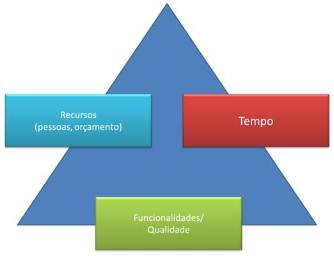
\includegraphics[scale=0.75]{pictures/restrictions_triangle.jpg}
\caption{Triângulo de Prioridades}
\label{Prioridades}
\end{figure}

A figura acima apresenta o triângulo de prioridades com as três prioridades principais do projeto. O projeto estará focado no tempo e qualidade, os recursos já estão definidos previamente, então não serão adqueridos novos recursos ao longo do desenvolvimento do projeto. Com relação ao tempo o projeto terá uma duração de 4 meses, ou seja, o desenvolvimento deverá correr rápido para que a equipe consiga entregar o jogo no prazo estipulado, porém, a qualidade não pode ser deixada de lado e o grupo buscará a melhor qualidade possível. 
Mesmo com o curto prazo de desenvolvimento o jogo deverá conter também muitas funcionalidades, deverá conter ao menos 5 missões jogáveis e completamente desenvolvidas para os usuários finais.

\section{Plataformas}

Inicialmente o jogo deverá ser capaz de rodar em um PC para os sistemas Linux e Windows. Posteriormente o mesmo poderá se aplicar para outras plataformas.

\section{Público-alvo}

O público alvo será para os maiores de 12 anos. O jogo conterá atos violentos, presença de sangue, exposição de cadáveres, etc.

\section{Estratégia de divulgação}

A principal estratégia de divulgação do jogo será a publicação do mesmo na Steam, para vendas online.

\section{Recursos disponíveis e Custos}

Os recursos disponíveis para o desenvolvimento contam com uma equipe de 8 pessoas, sendo 4 desenvolvedores, 3 artistas e um músico, também contam os equipamentos usados por cada membro da equipe. A seguir é apresentada uma tabela com os dados financeiros relacionados aos recursos disponíveis.

\begin{table}[h]
\begin{tabular}{|l|l|l|l|l}
\cline{1-4}
\multicolumn{1}{|c|}{\textbf{Recursos}} & \multicolumn{1}{c|}{\textbf{Quantidade}} & \multicolumn{1}{c|}{\textbf{Valor Unitário}} & \multicolumn{1}{c|}{\textbf{Valor Total}} &  \\ \cline{1-4}
Notebooks                               & 8                                        & R\$ 2300,00                                  & R\$ 18400,00                              &  \\ \cline{1-4}
Sublime Text 3                          & 4                                        & R\$ 212,10                                   & R\$ 848,40                                &  \\ \cline{1-4}
Cubase Pro 8                            & 1                                        & R\$ 323.59                                   & R\$ 323.59                                &  \\ \cline{1-4}
Audacity                                & 1                                        & R\$ 0,00                                     & R\$ 0,00                                  &  \\ \cline{1-4}
Linux                                   & 5                                        & R\$ 0,00                                     & R\$ 0,00                                  &  \\ \cline{1-4}
Windows 8                               & 3                                        & R\$ 359,00                                   & R\$ 1077,00                               &  \\ \cline{1-4}
*Adobe Ilustrator CC                    & 2                                        & R\$ 176,00                                   & R\$ 352,00                                &  \\ \cline{1-4}
*Adobe Photoshop CC Fotografia          & 2                                        & R\$ 88,00                                    & R\$ 176,00                                &  \\ \cline{1-4}
Publicação na Steam                     & 1                                        & R\$ 303,00                                   & R\$ 303,00                                &  \\ \cline{1-4}
\multicolumn{3}{|c|}{\textbf{Total}}                                                                                              & R\$ 21479,99                              &  \\ \cline{1-4}
\end{tabular}
\caption {Recursos de Hardware e Software}
\end{table}

\textit{* Os valores desses produtos são pagos por mês, a conta já converte o valor para 4 meses de uso.}
\newpage

\begin{table}[h]
\begin{tabular}{|l|l|l|l|l}
\cline{1-4}
\multicolumn{1}{|c|}{\textbf{Recursos}} & \multicolumn{1}{c|}{\textbf{Quantidade}} & \multicolumn{1}{c|}{\textbf{Valor Hora}} & \multicolumn{1}{c|}{\textbf{Valor Total}} &  \\ \cline{1-4}
Desenvolvedor                           & 4                                        & R\$ 21,51                                & R\$ 55065,60                              &  \\ \cline{1-4}
Designer Gráfico                        & 3                                        & R\$ 11,94                                & R\$ 22924,80                              &  \\ \cline{1-4}
Músico                                  & 1                                        & R\$ 8,35                                 & R\$ 5344,00                               &  \\ \cline{1-4}
\multicolumn{3}{|c|}{\textbf{Total}}                                                                                          & R\$ 83334,40                              &  \\ \cline{1-4}
\end{tabular}
\caption {Recursos Humanos}
\end{table}

\textit{* Todos os valores foram calculados considerando-se 40 horas de trabalho semanais em 4 meses de trabalho.}
\textit{Fonte de Pesquisa: \url{http://www.salariobr.com/}}
\\

Valor total do projeto: {\textbf{R\$ 104.814,39.}}

\section{Lucro esperado}

A equipe espera alcançar um lucros perto de 25\% em cima dos valores gastos para o desenvolvimento do jogo, para isso, é necessário se alcançar um valor em torno de R\$ 130.000,00 nas vendas, deixando assim todas as dívidas quitadas e mais R\$ 25.185,61 líquido.

\section{Número estimado de cópias a serem vendidas}

A seguir é apresentada uma tabela com determinados preços para o jogo e o número estimado de cópias que deveriam ser vendidas para se alcançar os lucros esperados.

\begin{table}[h]
\begin{tabular}{|l|l|l|l|l}
\cline{1-4}
\multicolumn{1}{|c|}{\textbf{Valor do Jogo}} & \multicolumn{1}{c|}{\textbf{5 mil cópias vendidas}} & \multicolumn{1}{c|}{\textbf{10 mil cópias vendidas}} & \multicolumn{1}{c|}{\textbf{15 mil cópias vendidas}} &  \\ \cline{1-4}
R\$ 10,00                                    & R\$ 50.000,00                                        & R\$ 100.000,00                                        & R\$ 150.000,00                                     &  \\ \cline{1-4}
R\$ 15,00                                    & R\$ 75.000,00                                        & R\$ 150.000,00                                        & R\$ 225.000,00                                     &  \\ \cline{1-4}
R\$ 20,00                                    & R\$ 100.000,00                                       & R\$ 200.000,00                                        & R\$ 300.000,00                                     &  \\ \cline{1-4}
R\$ 25,00                                    & R\$ 125.000,00                                       & R\$ 250.000,00                                        & R\$ 375.000,00                                     &  \\ \cline{1-4}
R\$ 30,00                                    & R\$ 150.000,00                                       & R\$ 300.000,00                                        & R\$ 450.000,00                                     &  \\ \cline{1-4}
\end{tabular}
\caption{Valores alcançados de acordo com o valor do jogo}
\end{table}

Pode-se notar na tabela com os valores apresentados as opções possíveis para as vendas do jogo. Para quitar os gastos do projeto com uma meta de vendas para 5 mil cópias, o jogo deverá ter um valor de R\$ 21,00. Com uma expectativa de 10 mil cópias vendidas já fica possível um faixa de preço entre R\$ 10,00 e R\$ 15,00. Para se alcançar o valor esperado de R\$ 130.000,00 o jogo deveria ser vendido a R\$ 13,00 em uma expectativa de 10 mil cópias ou R\$ 26,00 visando 5 mil cópias vendidas.
\end{document}
